\documentclass{article}

\usepackage{graphicx}
\usepackage[shortlabels]{enumitem}
\usepackage{url}


\newcommand{\twopartdef}[4]
{
    \left\{
    \begin{array}{ll}
        #1 & #2 \\
        #3 & #4
    \end{array}
    \right.
}

\newcommand{\threepartdef}[6]
{
    \left\{
    \begin{array}{ll}
        #1 & #2 \\
        #3 & #4 \\
        #5 & #6
    \end{array}
    \right.
}

\begin{document}

\title{Time Range Queries for Hereditary Properties \\ \large 6.854 Final Project}
\author{Arsen Mamikonyan\thanks{arsen@mit.edu}, Hayk Saribekyan\thanks{hayks@mit.edu}}

\maketitle

\begin{abstract}
    Time range queries are important for analysing large datasets
    with timestamps. Such datasets are common in computational
    geometry, where a sequence of points with timestamps often
    corresponds to a trajectory of an object. Time range queries
    in this case check a certain property of section of the trajectory.

    In this paper we review recent general frameworks that can be
    used to handle property testing queries for time ranges, and
    discuss their implementations for solving certain problems in
    computational geometry. The results are limited to \textit{hereditary}
    properties, which cover a large variety of interesting problems.

    For two different hereditary properties, we compared the
    performance of efficient an algorithm and a naive one in practice.
    We observed that the efficient algorithms require more than ten
    times the amount of code in certain cases, but the large constant
    factor associated with it is compensated when working with large
    datasets.
\end{abstract}

\section{Introduction}
\label{sec:intro}

With the abundance of GPS and other movement tracking sensors there
is a large amount of timestamped location data.  This has led to
an increasing interest in geometric algorithms dealing with trajectory
analysis \cite{buchin2011finding, gudmundsson2007efficient,
aronov2016segmentation}.  In this work we focus on implementation
and analysis of two such algorithms dealing with hereditary properties
\cite{bokal2015, chan2016}.

The movement of an object in space can be modelled by a sequence
of points $S = s_1, \dots, s_n$. To analyse the trajectory of the
movement, one may want to check a certain property $P$ for portions
$S[i, j] = s_i, \dots, s_j$ of $S$ for given values of $i$ and $j$.
This paper discusses how to efficiently address such queries when
$P$ satisfies the following two properties:
\begin{itemize}
    \item $P$ is boolean.
    \item $P$ is hereditary. This means that for a given sequence
    $S$, if $P(S)$ is true, then $P(S')$ is true for any continuous
    subsequence $S'$ of $S$.
\end{itemize}

In this paper we discuss and implement two properties for a sequence of points $S = s_1, \dots, s_n$:
\begin{itemize}
    \item \textit{Monotonicity}:  $S$ is \textit{monotone} if there
    is a direction vector $v$ such that all vectors $\vec{(s_i,
    s_{i+1})}$ have a positive projection on $v$. In terms of
    trajectories, monotonicity shows whether the object travelled
    more or less in the same direction.
    \item \textit{Closeness}: $S$ is \textit{close} if any pair of
    points in $S$ is at most of distance $1$. One could use closeness
    queries to detect if a moving object mostly stayed in the same
    surrounding.
\end{itemize}

For a property $P$ satisfying the restrictions above, let $j^*(i)$
be the largest index $j$ such that $P$ holds for $S[i, j^*(i)] =
s_i, \dots, s_{j^*(i)}$. Now notice, that since $P$ is a hereditary
property $P(S[i, j]) = true$ if and only if $i \leq j \leq j^*(i)$.
Therefore, if we construct $j^*(i)$ we can answer property testing
queries in $O(1)$. Therefore, for the rest of the paper our goal
will be to efficiently compute $j^*(i)$.

Bokal et al. \cite{bokal2015} propose an algorithms that compute
$j^*(i)$ in $O(n)$ time for monotonicity, and in $O(n\log^2 n)$
time for closeness. Chan and Pratt \cite{chan2016} describe a
different algorithm to achieve the same result for closeness, but
also improve it to $O(n\log n)$ using fractional cascading.

The rest of the paper is organized as follows: Section \ref{sec:naive}
describes the naive algorithms we developed to solve two problems;
in Section \ref{sec:monotonicity} we review the general framework
that is set in \cite{bokal2015} for solving time range query problems,
and show how it is applied to compute $j^*(i)$ for monotonicity.
Section \ref{sec:closeness} reviews the framework by \cite{chan2016}
and its application for the closeness property. We then give some
implementation details in Section \ref{sec:implementation}, and
describe the experimental setup and our tests in Section
\ref{sec:experiments}.

\section{Naive Algorithms}
\label{sec:naive}
Suppose that for a sequence of length $n$ a property $P$ can be
checked in $T_P(n)$ time. Then, one can compute $j^*(i)$ using
binary search for each $i$. On a step of a binary search concerning
a range $[l, r]$ the algorithm would spend $T_P(r - l)$ time. The
total runtime of this simple algorithm is $O(nT_P(n)\log n)$. Call
this algorithm $SN$ (stands for super-naive). For the problems of
monotonicity and closeness we can do better.

\subsection{Monotonicity}
\label{sec:naive:monotonicity}
To detect whether a sequence is monotone or no, we can process the
points while keeping a set of polar angles (field-of-view or FoV)
that a direction vector $v$ can have. Notice that the FoV is always
an interval. When a new point arrives we can update the FoV in
constant time. If the FoV ever becomes empty, then the given sequence
is not monotone. This algorithm runs in $O(n)$ time for a sequence
of length $n$. Using this submodule for $SN$ we would get a $O(n^2\log
n)$ algorithm for computing $j^*(i)$ for all values of $i$.

However, doing a binary search for monotonicity is redundant, since
we will do the same computation many times. Instead, for each $i$
proceed with the FoV computation until it is empty, which will
happen precisely when we reach $j^*(i) + 1$. The resulting algorithm
runs in $O(n^2)$ time.

\subsection{Closeness}
\label{sec:naive:closeness}
The simple method of closeness-check takes $O(n^2)$ for a sequence
of $n$ points, because one has to check all pairs of points. This
results in $SN$ runtime of $O(n^3\log n)$, which is super-slow. We
can improve the closeness-check to $O(n\log n)$ using furthest-point
Voronoi diagrams, but that would not qualify for $SN$ and would
also take $O(n^2 \log^2 n)$ time to compute, which is also not fast.

Define $k^*(i)$ as the largest index such that $d(s_i, s_j) \leq
1$ for all $j \leq k^*(i)$. Clearly, $k^*(i) \geq j^*(i)$ because
we are checking for a weaker property. Also, notice that $k^*$ can
be computed in $O(n^2)$ for all points by calculating all pairwise
distances.

Noticing that 
\begin{equation}
\label{kj_rel}
j^*(i) = \min( j^*(i + 1), k^*(i) )
\end{equation}
we can calculate
$j^*(i)$ for all points in $O(n)$ extra time if we are given all
values for $k^*(i)$. So we found a $O(n^2)$ algorithm for computing
closeness property for all subsequences.

\section{Monotonicity in Linear Time}
\label{sec:monotonicity}
Bokal et al. introduced an elegant framework to deal with range
queries for hereditary problems. The key idea in their work is to
greedily split the given set of points into ranges, defined by
anchor points, and solve for each using a divide and conquer. To
simplify the reasoning we first define a property matrix $A_P$ such
that
\[ A_P(i, j) = \twopartdef{1}{P(S[i, j]) = true}{0}{P(S[i, j]) = false} \]

See Figure \ref{fig:property_matrix} for an example. Suppose that
there is an algorithm $J_P$ that, for a given $i$, finds $j^*(i)$
(notice that even if such $J_P$ exists, we are not happy to run it
$n$ times for each $i$). We use $J_P$ to find \textit{anchor} points
in $S$ as follows. Let $a_k$ be the index of $k^{th}$ anchor point
in $S$. We define $a_1 = s_1$, $a_k = \max(1 + a_{k-1}; j^*(a_{k-1}))$
for $k > 1$. Thus, the anchor points can be found using $J_P$.
Figure \ref{fig:property_matrix} shows the anchor points on $A$
(leftmost image).

\begin{figure}
    \centering
    \makebox[\textwidth][c]{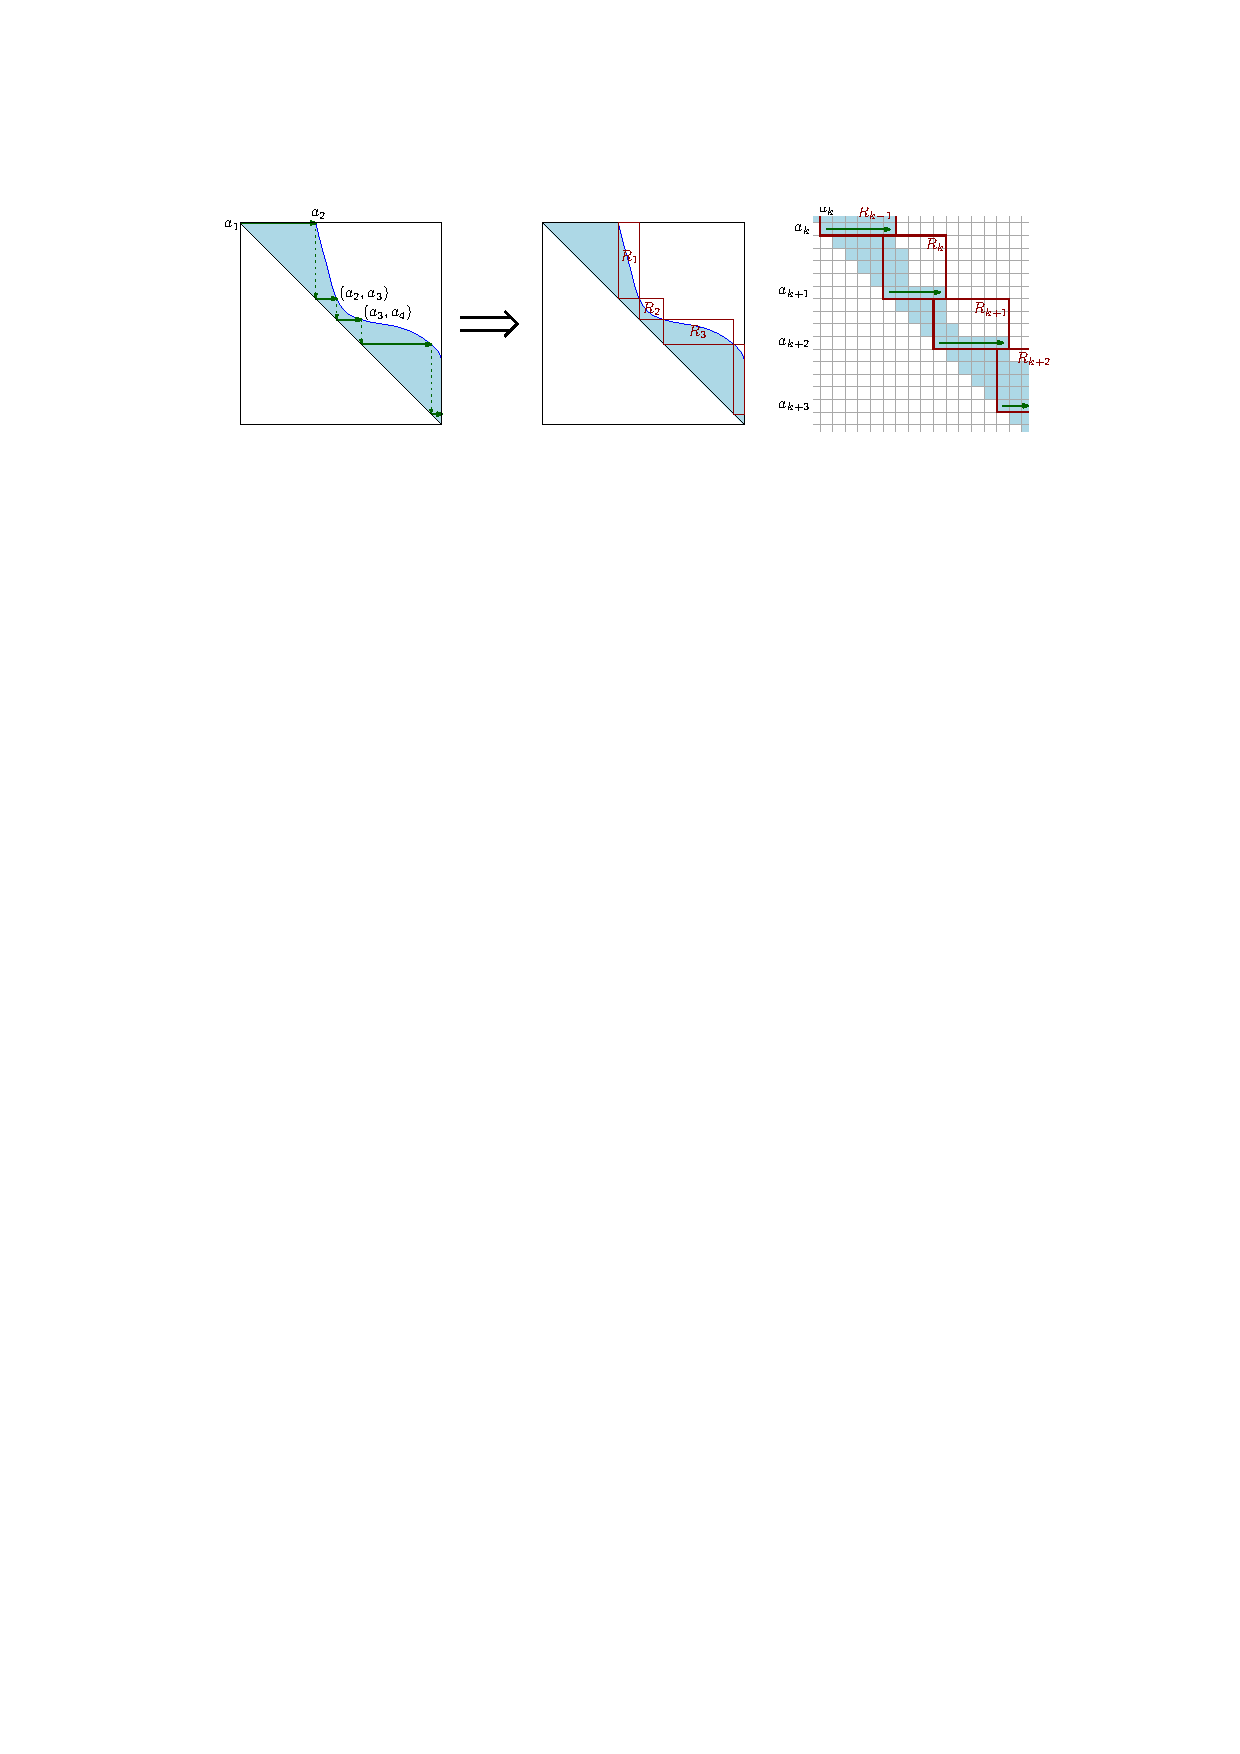
\includegraphics[width=1.1\textwidth]{figures/property_matrix.pdf}}
    \label{fig:property_matrix}
    \caption{The property matrix $A_P$. The blue regions show the
    locations that are 1. The left image illustrates the anchor
    points. The middle one shows the greedily constructed rectangles
    from the anchor points. On the right side is the detailed view
    of the property matrix. Figure from \cite{bokal2015}.}
\end{figure}

Also shown in Figure \ref{fig:property_matrix} are rectangles formed
using the anchor points. If we solve a rectangle (find the curve
in $A$ separating 1's from 0's) for each rectangle, then we will
be done, as stated in Lemma 2.1 from Bokal et al.

\textbf{Lemma 2.1 [Bokal et al.]:} Assume that we have the following two subroutines for sequence $S$ and a property $P$:
\begin{enumerate}[(a)]
    \item For any $a = 1, \dots, n$ find the $j^*(a)$, taking $T_{greedy}(j^*(a) - a)$
    \item Solve a rectangle with anchor points at opposite vertices (anchored rectangles). Suppose this module takes $T_{rect}(height(R) + width(R))$.
\end{enumerate}
Then we can solve the problem (i.e. find all $j^*(i)$) in time $O(n) + T_{greedy}((n)) + T_{rect}(n)$.

Both of these modules are property specific, but Bokal et al. make
another interesting generic step that explains how solving rectangles
can be done using a divide-and-conquer approach. We will, however,
skip that step and focus on the problem of monotonicity. It turns
out that monotonicity does not require the divide-and-conquer
approach to solve anchored rectangles.

\subsection{Solving Monotonicity}
Section \ref{sec:naive:monotonicity} discusses how to find $j^*(i)$
in linear time for a given $i$ by using intervals of polar angles.
This algorithm will serve as the subroutine for Lemma 2.1(a).

Consider an anchored rectangle $R$ with a lower-left corner $(a, a)$, width $w$ and height $h$.
\begin{enumerate}[-]
	\item By traversing the points $S[a, a + w]$, we can compute
	for each $j = a, \dots, a + w$ the interval of polar angles
	$I_j$ such that $S[a, j]$ is monotone with respect to all
	directions in $I_j$.
	\item By traversing the points $S[a - h, a]$ in reverse
	order, a similar set $I_i$ can be computed for $a - h \leq
	i < a$, representing the set of monotone directions for
	$S[i, a]$.
\end{enumerate}

If $i < a < j$, then $S[i, j]$ is monotone if and only if $I_i$ and
$I_j$ have a non-empty intersection. Thus, for each $i = a - h,
\dots, a$, $j^*(i)$ is the largest index such that $I_i \cap
I_{j^*(i)} \neq \emptyset$.  Noting that search for $j^*(i+1)$ can
start from $j^*(i)$, we can compute $j^*(i)$ for all $i \in [a -
h, a]$ in linear time.

These two subroutines, together with Lemma 2.1 give a linear solution
to the monotonicity problems. We have evaluated Naive algorithm
(from Section \ref{sec:naive}) and this algorithm in Section
\ref{sec:experiments}.

%This is where divide and conquer strategy is used. Consider a rectangle $R$ with rows $[a, a + h]$ and columns $[b, b + w]$. We can set $m = a + [h / 2]$ and using $J_P$ find $j^*(m)$. If $m \leq i \leq a + h$ then $j^*(i) \geq j^*(m)$, and if $a \leq i \leq m$ then $j^*(i) \leq j^*(m)$. Therefore, once we know the value of $j^*(m)$ the solution for $R$ can be computed using two recursive calls to its upper-left and lower-right sub-rectangles.

%Notice, however, this type of recursion will just end up calling $J_P$ for all indices in $[a, a + h]$, having no divide-and-conquer effect.

\section{Closeness in $O(n \log^2 n)$}
\label{sec:closeness}

Chan, Prat \cite{chan2016} take a different approach to calculating
hereditary properties, they first efficiently calculate $k^*$ values
for all the pairs using a range tree \cite{lueker1978data} that has
a secondary structure to make querying faster, and then they calculate
$j^*$ values from those.

During the first part of the algorithm we use a data structure
that given a point $i$, could efficiently answer what is the point
with smallest index $k^*(i)+1$ that lies outside a unit circle
centered at $i$. Notice that this is equivalent to checking whether
$s_i$ lines in the intersection of unit circles centered at points
$s_{i+1}, \dots, s_{k^*(i)}$. The intersection of unit circles is
convex and we call it \textit{polyarcs}, as it is similar to a
polygon, but has arcs of circles as edges instead of straight lines.
In order to check whether a point is inside a polyarc formed by a
range of points in the given sequence, we use a binary range tree.

\begin{figure}[h]
    \centering
    \makebox[\textwidth][c]{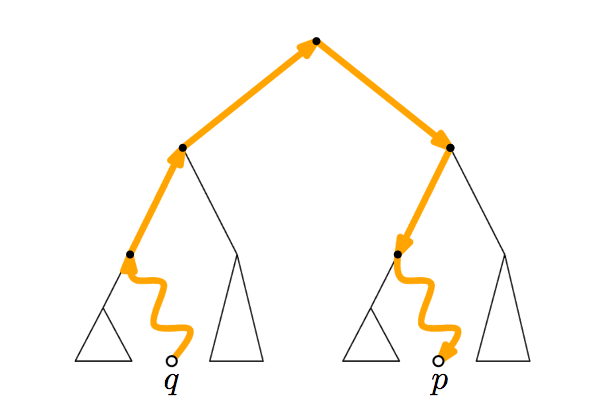
\includegraphics[width=0.5\textwidth]{figures/query_path}}
    \label{fig:query_path}
    \caption{A search path finding $p = k^*(q) + 1$ of point $q$.
    The search goes up until it find a range where $p$ lies and
    then goes down narrowing the range until it reaches the
    leaf $p$.
    Figure from \cite{chan2016}.}
\end{figure}

First we build a regular 1 dimensional range tree using indices of
the data points. Each node $v$ of the range tree represents a
continuous interval of a given points, and stores the polyarc that
is formed by intersecting unit circles centered at these points.

Suppose we have an algorithm that can test whether a point is inside
a polyarc in $Q(n)$ time. Then using the range tree we can find
$k^*(i)$ for any point in $O(Q(n)\log n)$ time using the following
algorithm. It starts the search from a leaf corresponding to the
query point $q$ (see Figure 2).
% NOTE: latex messes up Figure number, so hardcode it for now!

\begin{enumerate}[-]
\item
In the first ``up'' phase, we walk upward from $q$ towards the root.
Each time we go up from a left child, we query the secondary structure
at right sibling, to see if there exists a point in that range that
is far from $q$.
\begin{itemize}
\item If no, we can extend the search by going one more level up.
\item If yes, the first point far from $q$ is in the right child,
so we proceed to the second step to locate that node.
\end{itemize}


\item In the second (``down'') phase, we walk downward from the
current node to a leaf to locate the far point with smallest index.
Each time we descend from a node, we query the secondary structure
at the left child to see if there exists a point in the left child's
range that is far from $q$
\begin{itemize}
\item If no, the point that's far from $q$ lies in the range of the
right child, so we descend right.
\item If yes, we descend left.
\end{itemize}
\end{enumerate}

After we find $k^*(i)$ for all the nodes, we combine those using
Equation \ref{kj_rel} in $O(n)$ time to find $j^*(i)$ for all $i$.
This gives total runtime of $O(n \log n Q(n))$.

Now, to compute the intersection of polyarcs we use a relatively
standard technique. It is possible to extend the sweep-line polygon
intersection algorithm by Shamos and Hoey \cite{shamos1976geometric},
for computing polyarc intersections in linear time, assuming that
the vertices of the shapes are given in sorted order. We can construct
the range-tree from bottom to up, at each level spending $O(n)$
time to intersect all polyarcs on that level. Therefore, the total
construction time of a range tree is $O(n \log n)$.

By storing the vertices of the polyarcs in sorted order with respect
to their $x$ coordinate we can answer \textit{contains} queries in
$Q(n) = O(\log n)$ time using a binary search. This gives us an
$O(n\log^2 n)$ algorithm to compute $j^*(i)$ for all $i$. The next
section contains the details about the implementation of this
algorithm.

\section{Implementation Details}
\label{sec:implementation}
In the papers reviewed here (\cite{bokal2015,chan2016}) there are
at least 6 algorithms presented. We wanted to implement algorithm
that use frameworks of both papers. In order to limit the size of
the implementation we decided to pick monotonicity property for its
simplicity (and elegance), which was solved in Bokal et al.
\cite{bokal2015}. We chose to implement the closeness testing
algorithm from \cite{chan2016} because it used many ideas from the
class, for example the intersection of convex envelopes in 2
dimensions, range trees.

The implementations of naive algorithms as well as of the efficient
monotonicity testing algorithm are relatively easy, so in this paper
we skip discussing them. We implemented the $O(n \log ^2 n)$ algorithm
for solving closeness testing from \cite{chan2016}.  The algorithm
has two distinct parts: a high-level tree-range data structure, and
a lower-level data structure for storing \textit{polyarcs} (see
Section \ref{sec:closeness}).  Higher level algorithm was easier
of the two, it involved implementing a range tree and the querying
algorithm described in Section \ref{sec:closeness}.

A polyarc is a convex geometric shape, which is defined by a clockwise
set of its vertices like a polygon. Unlike a polygon, each edge of
a polyarc is an arc of a circle. The algorithm needs to be able to
find the intersection of two polyarcs, and also decide whether a
query point is inside the polyarc.

Both of these algorithms are similar to those of polygons, but the
majority of the implementation effort was spent to handle the cases
specific to polyarcs. Our representation of polyarcs has two
``sides'': upper and lower, respectively the upper part of the
complex shape and the lower one. To intersect two polyarcs we first
find a minimal upper envelope i.e. for each $x$ coordinate we
recorded the polyarc that had a lower upper side. Similarly, we
computed a maximal lower envelope. The area above the maximal lower
envelope and minimal upper envelope is the intersection of two
polyarcs. Each of these steps can be performed in linear time by a
sweep line technique.

The envelope representation of polyarcs is also helpful for querying
whether a point is inside the polyarc or no. One needs to simply
do a binary search for the $x$ coordinate of the candidate point.
If a vertical line at that location crosses the higher envelope on
a larger value of $y$ than the lower envelope, then the query point
is inside the polyarc.

Overall, we wrote more than 1200 lines of code in C++ for the
implementation of the algorithms \cite{report_code}, and 800 lines
of code for testing. Large part of the code is dedicated to the
closeness algorithm in $O(n \log^2 n)$. We used C++ for the
implementation so that the overhead that the language adds to the
runtime is minimized. A simple language to write code in is Python,
but we think that in this case the strong type checking of C++
helped us, because of a complex structure of the code.

\section{Experimental Results}
\label{sec:experiments}
We have tested the performance of the algorithms we've implemented
with synthetic datasets, which we tried to model based on some
potential problems where the algorithms could have been used.
% - mention that we have used random walk to mimic reality. in that case the good algorithm for monotonicity is not that good. but for the worst case, it's great.
% - 

\subsection{Monotonicity}
\label{sec:experiments:monotonicity}

\begin{figure}[!ht]
  \centering
  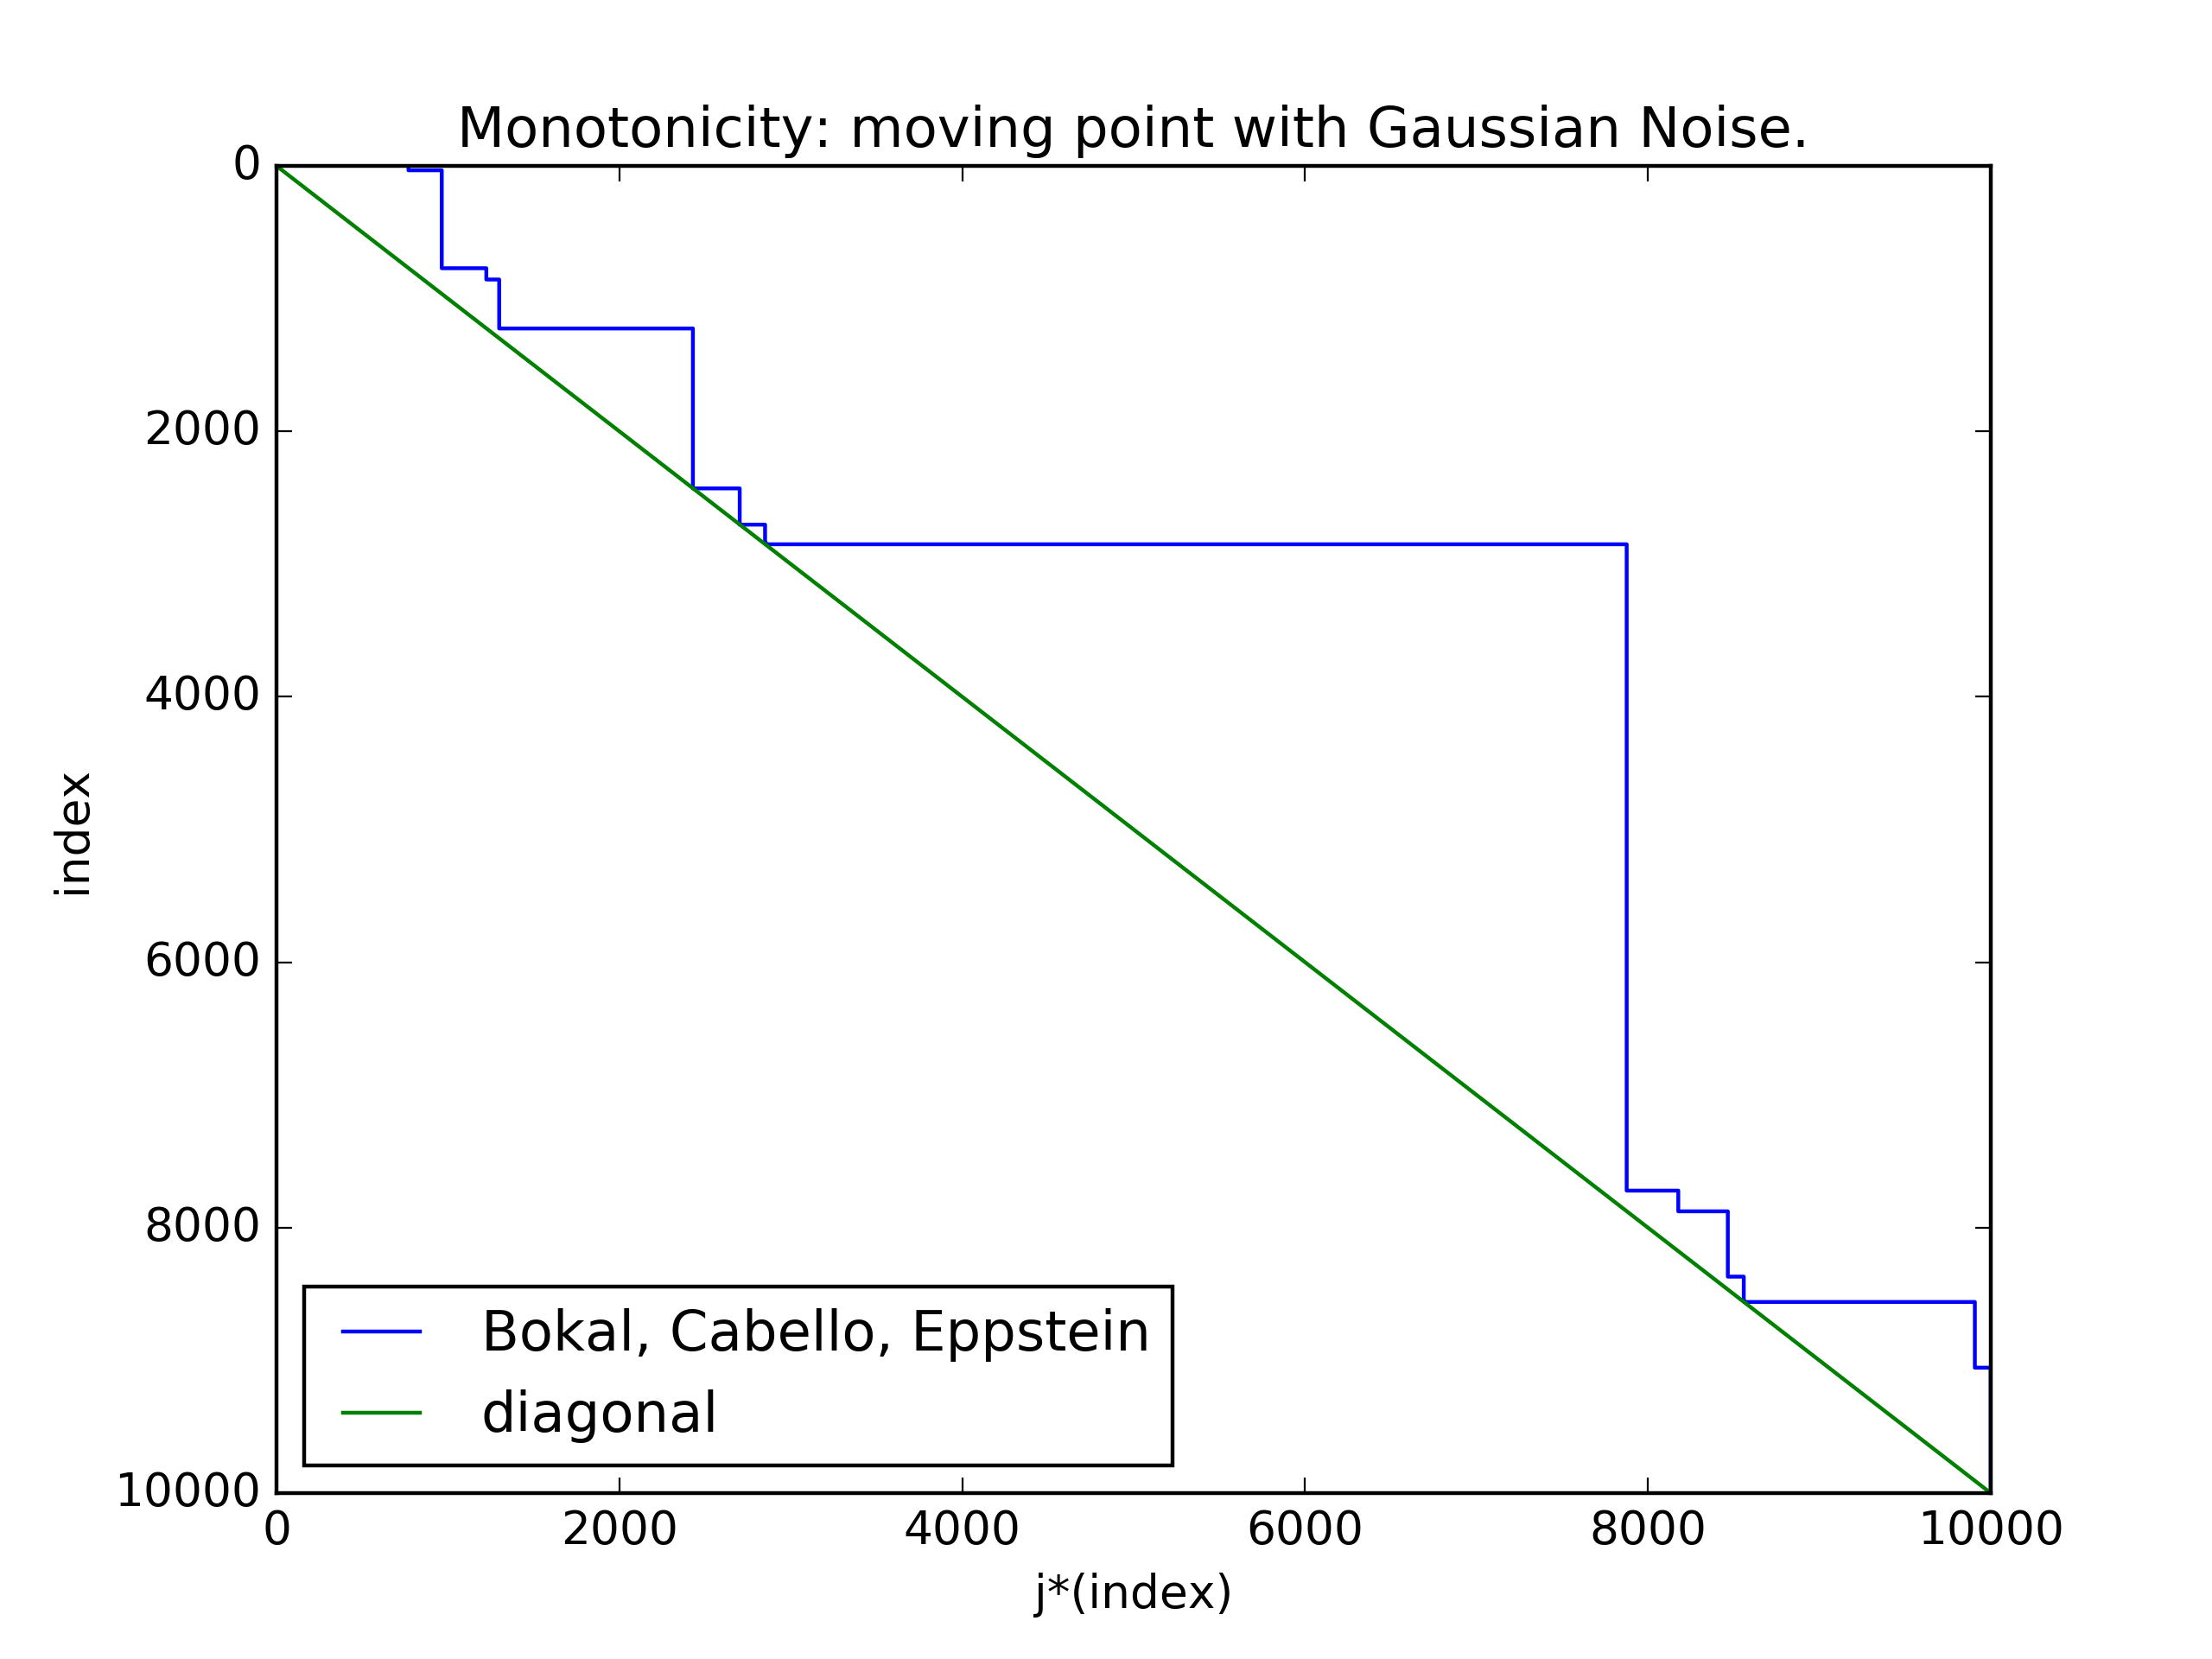
\includegraphics[height=8cm]{../plots/monotonicity_moving_gaussian}
  \caption{Property matrix for movement monotonicity for time intervals for a point moving steadily in $x$ direction with Gaussian noise with $\sigma_x = 0.05, \sigma_y = 1$. Average value of $j^*(i) - i = 1520$}
  \label{fig:monotonicity_demo}
\end{figure}

\begin{figure}[!ht]
    \centering
    \begin{tabular}{c|c|c}
        points in dataset & Bokal et al. & Naive  \\
    \hline
        1000    & 0.6    & 3.6  \\
    \hline
        3333    & 2.1    & 12.8  \\
    \hline
        10000    & 5.8    & 43.5  \\
    \hline
        33333    & 19.3    & 142.2  \\
    \hline
        100000    & 64.2    & 416.8  \\
    \hline
        333333    & 202.0    & 1,398.2  \\
    \end{tabular}
    \caption{Runtimes (in milliseconds) of \textbf{monotonicity}
    algorithms Naive and Bokal et. al for \textbf{moving point} in
    $x$ direction with Gaussian noise. Mean value of $j^*(i) - i =
    1520$ for 10,000 points.}
    \label{fig:monotonicity_comparison_moving_gaussian}
\end{figure}

\begin{figure}[!ht]
    \centering
	\begin{tabular}{c|c|c}
	    points in dataset   & Bokal et al. & Naive  \\
	\hline
	    3000    & 1.9    & 2.6  \\
	\hline
	    10000    & 6.0    & 8.3  \\
	\hline
	    30000    & 18.0    & 25.0  \\
	\hline
	    100000    & 61.7    & 89.5  \\
	\hline
	    300000    & 190.5    & 258.3  \\
	\hline
	    1000000    & 629.5    & 909.6 
	\end{tabular}
    \caption{Runtimes (in milliseconds) of \textbf{monotonicity}
    algorithms of Naive and Bokal et. al for \textbf{random walk}
    dataset. Mean value of $j^*(i) - i = 4.0$ for 10,000 points.}
    \label{fig:monotonicity_comparison_random_walk}
\end{figure}

For monotonicity we have tried looking at a trajectory of a particle
moving steadily along $x$ axis, but with some noise added to the
movement. This datasets models a typical problem where we want to
find for how long the particle moves monotonically. The goal is to
find all subsequences of intervals that the trajectory had some
constant direction. In Figure \ref{fig:monotonicity_demo} you can
see the property matrix (i.e. the region where the property holds)
when the noise added is a Gaussian noise with standard deviations
$\sigma_x = 0.05, \sigma_y = 1$. We chose these characteristics of
the noise to have an interesting looking property matrix, where the
average length of longest subsequence is 1520 (vs 5000 if there was
no noise).

You can see that the area of the region where the property is
substantial, so we expect Naive algorithm to perform worse than the
faster version that we've implemented.  Figure
\ref{fig:monotonicity_comparison_moving_gaussian} shows runtime
differences in milliseconds between Naive algorithm and algorithm
we presented from Bokal et al. From the runtime we can see that
Bokal et al. clearly outperforms the Naive algorithm.

If we were to look at a different dataset, e.g. a random walk, the
performance results could be different. Figure
\ref{fig:monotonicity_comparison_random_walk} shows that the runtimes
of the two algorithms are actually very close in practice for this
case. This happens because the property matrix has few \textit{true}
values, in this case average value of $j^*(i) - i = 4.0$, so naive
algorithm performs very few comparisons, whereas Bokal et al. still
have to build the range tree with all the auxiliary data structures
on all the nodes.


\subsection{Closeness}
\label{sec:experiments:closeness}


\begin{figure}[!ht]
  \centering
  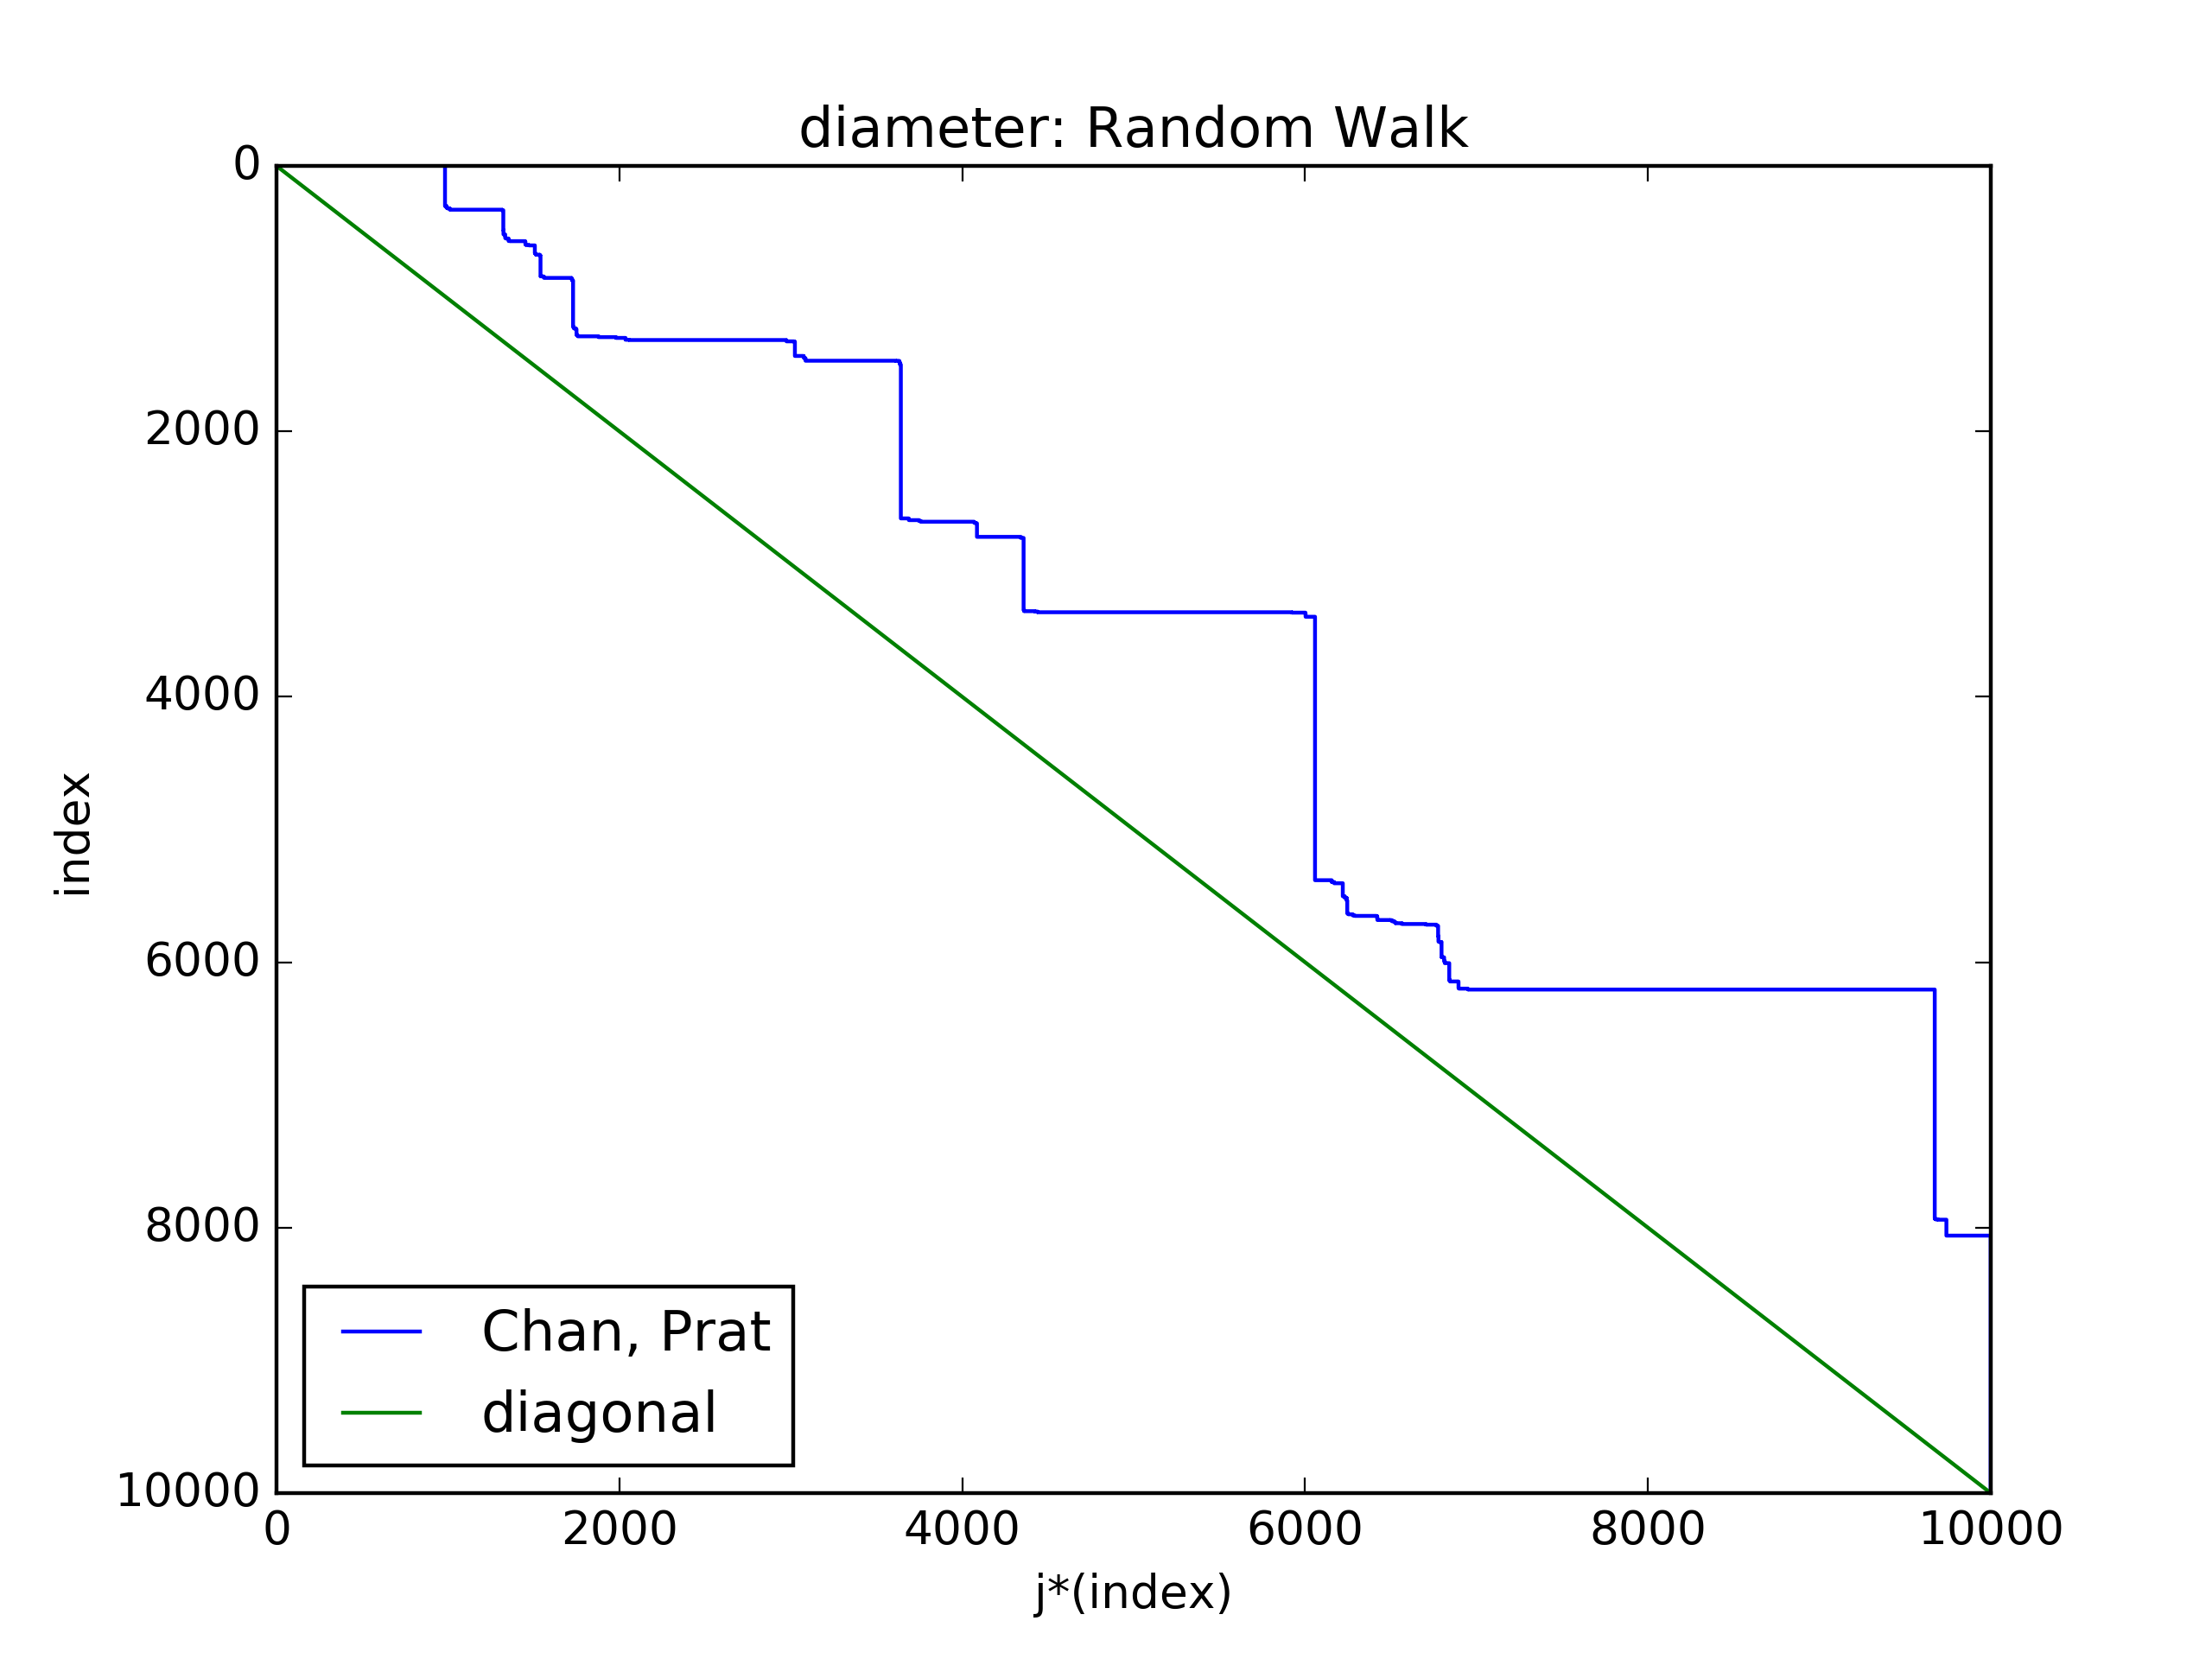
\includegraphics[height=8cm]{../plots/diameter_random_walk}
  \caption{Property matrix for checking 1 distance \textbf{closeness}
  on a random walk with step size 0.3. Average value of $j^*(i) - i = 1013$}
  \label{fig:diameter_demo}
\end{figure}

\begin{figure}[!ht]
  \centering
\begin{tabular}{c|c|c}
    points in dataset &  Chan Prat    & Naive  \\
\hline
    1000    & 9.3    & 0.5  \\
\hline
    3333    & 28.3    & 1.5  \\
\hline
    10000    & 88.7    & 4.5  \\
\hline
    33333    & 307.1    & 15.5  \\
\hline
    100000    & 815.2    & 46.8  \\
\hline
    333333    & 2,736.9    & 157.3 
\end{tabular}
  \caption{Runtimes (in milliseconds) of \textbf{closeness} algorithms
  Naive and Chan, Prat on \textbf{moving point} datasets. Mean value
  of $j^*(i) - i = 0.16$ for 10,000 points.}
  \label{fig:diameter_comparison_moving_gaussian}
\end{figure}

\begin{figure}[!ht]
  \centering
\begin{tabular}{c|c|c}
    points in dataset &  Chan/Prat    & Naive  \\
\hline
    3000    & 79.3    & 1,316.2  \\
\hline
    10000    & 269.7    & 5,998.3  \\
\hline
    30000    & 886.3    & 26,716.6  \\
\hline
    100000    & 2,751.2    & 90,934.6 
\end{tabular}
  \caption{Runtimes (in milliseconds) of \textbf{closeness} algorithm
  Naive and Chan, Prat on \textbf{random walk} datasets. Mean value
  of $j^*(i) - i = 1013$. for 10,000 points. We have included less
  data points because runtime of Naive algorithm became too large.}
  \label{fig:diameter_comparison_random_walk}
\end{figure}

For testing the closeness algorithm, we have generated points from
a random walk.  At each step we uniform randomly pick a direction,
and move 0.3 distance in that direction. And we want to know all
subsequences of the walk that are clustered together within distance
of 1.

Figure \ref{fig:diameter_demo} shows the property matrix when running
closeness algorithm on the random walk data. Again we have picked
the step size (0.3) to have a relatively high mean value for $j^*(i)
-i = 1013$.

Figure \ref{fig:diameter_comparison_random_walk} shows runtime
comparisons for different dataset sizes. Notice that Chan Prat
algorithm outperforms the Naive algorithm by a big margin, which
increases as number of points increase.

Whereas if we run the same algorithms on the dataset from Section
\ref{sec:experiments:monotonicity}, where we expect to have very
small values for closeness property, we see (Figure
\ref{fig:diameter_comparison_moving_gaussian}) that Naive algorithm
is doing better. This happens because building the range tree with
circle intersections costs $O(n \log n)$, whereas the expected
length of subsequence is much less than $\log n$, in case of $10,000$
points it equals to $0.16$

\section{Conclusion}
\label{sec:conclusion}

In this report we looked at two frameworks for testing queries for
time ranges\cite{bokal2015, chan2016}, and implemented each of the
frameworks for solving a corresponding hereditary property problem
\cite{report_code}. Besides implementing the frameworks we had to
implement other algorithms, e.g. sweep line and range trees, to
solve corresponding hereditary property problems.

We showed that both frameworks outperform simpler algorithms that
have worse theoretical bound on synthetic datasets that mimic real
life problems. We also showed that there is significant overhead
that comes with these frameworks and sometimes if the dataset is
simple naive algorithms outperform (or are equivalent) more
complex ones.

We learned that implementing computational geometry algorithms is
tricky because all the algorithms have a lot of edge cases, and
internal structure of data structures is very important to get the
algorithm right.

\bibliographystyle{unsrt}
\bibliography{papers}
\end{document}
